\section{Materiales}

\SectionPage

\begin{frame}{Materiales}

    Identificaremos cada elemento asignando un entero positivo \(id \in \mathbb{N}\) que será devuelto junto con la distancia a este objeto, es decir, vamos a devolver un \textit{vec2} cuya componente \enquote{x} será la distancia y cuya componente \enquote{y}, el identificador \(id\). Asignaremos la constante \(id=0\) cuando no se ha trazado ningún objeto. Esto hace que \(f\), nuestra escena, esté definida como,
    \[f:\mathbb{R}^3\longrightarrow\mathbb{R}\times\mathbb{N}\]
    El pixel resultado, será:
    \[ \text{color}_{rgb}(id) = \text{obtenerMaterial}(id) \cdot I_{Phong} \]

    También podemos utilizar el punto \(\Vec{p}\) y el identificador \(id\) para calcular la proyección hacia el sistema de coordenadas de alguna textura y tener así una escena más rica.

\end{frame}


\begin{frame}{Materiales}

    Utilizando la ecuación de la proyección cilíndrica:
    
    \[\begin{pmatrix}
    u&
    v
\end{pmatrix}=  0.5\cdot
\begin{pmatrix}
    \dfrac{\arctan\left(\dfrac{\Vec{p}_x}{\Vec{p}_z}\right)}{\pi}+1&
    \Vec{p}_y + 1
\end{pmatrix}
\]
    Se ha creado la siguiente imagen:
    
    \vfill
    
    \begin{figure}[H]
      \centering
      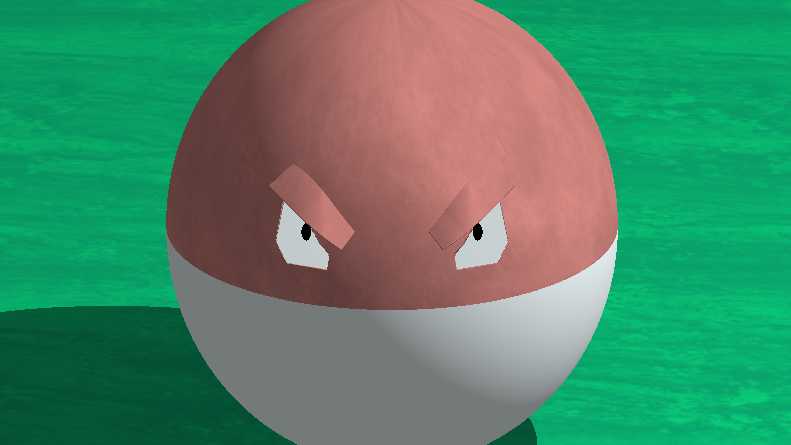
\includegraphics[width=0.5\textwidth]{imagenes/voltorb.png}
      {\url{https://www.shadertoy.com/view/wsGGWG}}
    \end{figure}

\end{frame}